% ============================================================
\chapter{Th\'eorie des Graphes Appliqu\'ee}
\label{ch:graphes}
% ============================================================

En 1736, Leonhard Euler se penche sur un probl\`eme r\'ecr\'eatif pos\'e par les habitants de K\"onigsberg~: peut-on traverser les sept ponts de la ville en ne passant qu'une seule fois sur chacun~? En prouvant que c'est impossible, Euler ne r\'esout pas seulement une \'enigme de promenade~: il fonde la th\'eorie des graphes, une branche des math\'ematiques qui deviendra indispensable \`a la recherche op\'erationnelle. Aujourd'hui, les graphes mod\'elisent les r\'eseaux de transport, les circuits \'electroniques, les r\'eseaux sociaux, les cha\^ines logistiques. Trouver le plus court chemin, l'arbre couvrant de co\^ut minimal, le flot maximal --- autant de probl\`emes fondamentaux dont les algorithmes (Dijkstra, Kruskal, Ford-Fulkerson) sont utilis\'es des millions de fois par jour dans les syst\`emes informatiques du monde entier.

\section{D\'efinitions fondamentales}

\begin{definition}[Graphe]
Un \textbf{graphe} $G = (V, E)$ est un couple o\`u $V$ est un ensemble fini
de \textbf{sommets} (ou n\oe uds) et $E$ un ensemble d'\textbf{ar\^etes}
(graphe non orient\'e) ou d'\textbf{arcs} (graphe orient\'e, not\'e
$G = (V, A)$).
\end{definition}

\begin{definition}[Graphe pond\'er\'e]
Un graphe est \textbf{pond\'er\'e} si chaque ar\^ete/arc $(i,j)$ est muni d'un
poids $w(i,j) \in \R$ (distance, co\^ut, capacit\'e, etc.).
\end{definition}

\begin{center}
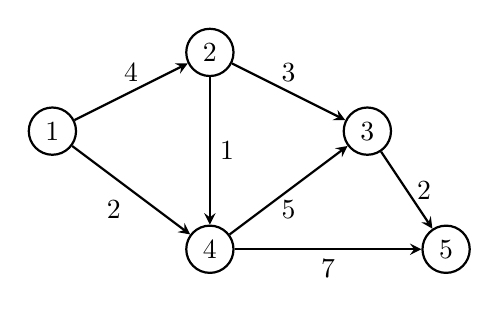
\begin{tikzpicture}[
    vertex/.style={circle, draw, minimum size=6mm, inner sep=0pt},
    >=stealth, thick
  ]
  \node[vertex] (1) at (0,2) {1};
  \node[vertex] (2) at (2,3) {2};
  \node[vertex] (3) at (4,2) {3};
  \node[vertex] (4) at (2,0.5) {4};
  \node[vertex] (5) at (5,0.5) {5};
  \draw[->] (1) -- node[above] {4} (2);
  \draw[->] (1) -- node[below left] {2} (4);
  \draw[->] (2) -- node[above] {3} (3);
  \draw[->] (2) -- node[right] {1} (4);
  \draw[->] (3) -- node[right] {2} (5);
  \draw[->] (4) -- node[below] {5} (3);
  \draw[->] (4) -- node[below] {7} (5);
\end{tikzpicture}
\end{center}

\begin{definition}[Chemin et cycle]
Un \textbf{chemin} de $u$ \`a $v$ est une suite de sommets
$u = v_0, v_1, \ldots, v_k = v$ tels que $(v_{i-1}, v_i) \in E$ pour tout
$i$.  Sa \textbf{longueur} est la somme des poids.  Un \textbf{cycle} est
un chemin ferm\'e ($u = v$) de longueur non nulle.
\end{definition}

\begin{definition}[Graphe connexe]
Un graphe non orient\'e est \textbf{connexe} s'il existe un chemin entre
toute paire de sommets.  Un graphe orient\'e est \textbf{fortement connexe}
s'il existe un chemin orient\'e entre toute paire ordonn\'ee de sommets.
\end{definition}

\begin{definition}[Arbre]
Un \textbf{arbre} est un graphe connexe sans cycle.  Il poss\`ede
exactement $\abs{V} - 1$ ar\^etes.
\end{definition}

\section{Repr\'esentation des graphes}

\begin{formules}[title=\textbf{Structures de donn\'ees}]
\begin{itemize}
  \item \textbf{Matrice d'adjacence} $A \in \{0,1\}^{n \times n}$~:
        $A_{ij} = 1$ si $(i,j) \in E$.  M\'emoire~: $\mathcal{O}(n^2)$.
  \item \textbf{Listes d'adjacence}~: pour chaque sommet, la liste de ses
        voisins.  M\'emoire~: $\mathcal{O}(n + m)$.
  \item \textbf{Matrice de poids} $W$~: $W_{ij} = w(i,j)$ ou $+\infty$
        si $(i,j) \notin E$.
\end{itemize}
\end{formules}

\section{Plus court chemin depuis une source unique}

\subsection{Algorithme de Dijkstra}

\begin{theoreme}[Condition d'application]
L'algorithme de Dijkstra calcule les plus courts chemins depuis un sommet
source $s$ dans un graphe \`a poids \textbf{non n\'egatifs} en temps
$\mathcal{O}((n + m) \log n)$ avec un tas binaire.
\end{theoreme}

\begin{algorithme}[title=\textbf{Algorithme de Dijkstra}]
\begin{enumerate}
  \item Initialiser $d[s] = 0$, $d[v] = +\infty$ pour $v \ne s$.
  \item $Q \leftarrow V$ (file de priorit\'e).
  \item Tant que $Q \ne \emptyset$~:
    \begin{enumerate}
      \item Extraire $u = \argmin_{v \in Q} d[v]$.
      \item Pour chaque voisin $v$ de $u$ avec $(u,v) \in E$~:
        si $d[u] + w(u,v) < d[v]$~:
        $d[v] \leftarrow d[u] + w(u,v)$, $\pi[v] \leftarrow u$.
    \end{enumerate}
\end{enumerate}
\end{algorithme}

\begin{exemple}[Dijkstra]
Sur le graphe ci-dessus avec source $s = 1$~:

\begin{center}
\begin{tabular}{c|ccccc}
  \'Etape & $d[1]$ & $d[2]$ & $d[3]$ & $d[4]$ & $d[5]$ \\
  \hline
  Init & 0 & $\infty$ & $\infty$ & $\infty$ & $\infty$ \\
  $u=1$ & 0 & 4 & $\infty$ & 2 & $\infty$ \\
  $u=4$ & 0 & 3 & 7 & 2 & 9 \\
  $u=2$ & 0 & 3 & 6 & 2 & 9 \\
  $u=3$ & 0 & 3 & 6 & 2 & 8 \\
  $u=5$ & 0 & 3 & 6 & 2 & 8 \\
\end{tabular}
\end{center}

Plus court chemin $1 \to 5$~: $1 \to 4 \to 3 \to 5$ de longueur 8.
\end{exemple}

\subsection{Algorithme de Bellman-Ford}

\begin{theoreme}[Bellman-Ford]
L'algorithme de Bellman-Ford calcule les plus courts chemins depuis $s$ en
pr\'esence de poids \textbf{n\'egatifs} (mais sans cycle n\'egatif accessible)
en temps $\mathcal{O}(nm)$.
\end{theoreme}

\begin{algorithme}[title=\textbf{Algorithme de Bellman-Ford}]
\begin{enumerate}
  \item Initialiser $d[s] = 0$, $d[v] = +\infty$ pour $v \ne s$.
  \item R\'ep\'eter $\abs{V} - 1$ fois~:
    \begin{enumerate}
      \item Pour chaque arc $(u,v) \in A$~: si $d[u] + w(u,v) < d[v]$~:
            $d[v] \leftarrow d[u] + w(u,v)$, $\pi[v] \leftarrow u$.
    \end{enumerate}
  \item \textbf{D\'etection de cycle n\'egatif}~: pour chaque arc $(u,v)$~:
        si $d[u] + w(u,v) < d[v]$, il existe un cycle n\'egatif.
\end{enumerate}
\end{algorithme}

\begin{attention}[title=\textbf{Cycles n\'egatifs}]
En pr\'esence d'un cycle n\'egatif accessible depuis $s$, la notion de plus
court chemin n'est pas d\'efinie (on peut faire $d \to -\infty$).
Bellman-Ford d\'etecte cette situation.
\end{attention}

\section{Plus courts chemins entre toutes les paires}

\begin{algorithme}[title=\textbf{Algorithme de Floyd-Warshall}]
Complexit\'e~: $\mathcal{O}(n^3)$.
\begin{enumerate}
  \item Initialiser $D^{(0)} = W$ (matrice de poids).
  \item Pour $k = 1, \ldots, n$~:
    \[
      D^{(k)}_{ij} = \min\left(D^{(k-1)}_{ij},\;
        D^{(k-1)}_{ik} + D^{(k-1)}_{kj}\right)
    \]
\end{enumerate}
\end{algorithme}

\section{Arbres couvrants minimaux}

\begin{definition}[Arbre couvrant minimal (ACM)]
Un \textbf{arbre couvrant minimal} d'un graphe connexe pond\'er\'e $G = (V, E)$
est un sous-graphe couvrant sans cycle de poids total minimal.
\end{definition}

\subsection{Algorithme de Kruskal}

\begin{algorithme}[title=\textbf{Kruskal}]
\begin{enumerate}
  \item Trier les ar\^etes par poids croissant.
  \item Pour chaque ar\^ete $(u,v)$ par ordre de poids~:
    \begin{enumerate}
      \item Si $u$ et $v$ sont dans des composantes diff\'erentes~:
            ajouter $(u,v)$ \`a l'ACM et fusionner les composantes
            (Union-Find).
    \end{enumerate}
  \item S'arr\^eter apr\`es $\abs{V} - 1$ ar\^etes.
\end{enumerate}
Complexit\'e~: $\mathcal{O}(m \log m)$.
\end{algorithme}

\subsection{Algorithme de Prim}

\begin{algorithme}[title=\textbf{Prim}]
\begin{enumerate}
  \item Choisir un sommet initial $s$.  $T \leftarrow \{s\}$.
  \item Tant que $\abs{T} < \abs{V}$~:
    \begin{enumerate}
      \item Trouver l'ar\^ete $(u,v)$ de poids minimal avec $u \in T$,
            $v \notin T$.
      \item Ajouter $v$ \`a $T$ et $(u,v)$ \`a l'ACM.
    \end{enumerate}
\end{enumerate}
Complexit\'e~: $\mathcal{O}((n + m) \log n)$ avec un tas binaire.
\end{algorithme}

\begin{exemple}[ACM par Kruskal]
\begin{center}
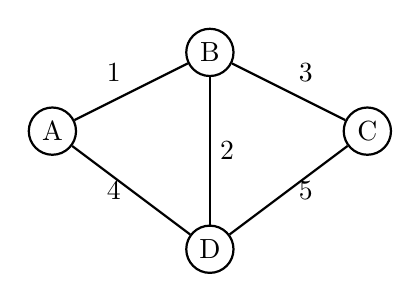
\begin{tikzpicture}[
    vertex/.style={circle, draw, minimum size=6mm, inner sep=0pt},
    thick
  ]
  \node[vertex] (A) at (0,2) {A};
  \node[vertex] (B) at (2,3) {B};
  \node[vertex] (C) at (4,2) {C};
  \node[vertex] (D) at (2,0.5) {D};
  \draw (A) -- node[above left] {1} (B);
  \draw (A) -- node[left] {4} (D);
  \draw (B) -- node[above right] {3} (C);
  \draw (B) -- node[right] {2} (D);
  \draw (C) -- node[right] {5} (D);
\end{tikzpicture}
\end{center}

Ar\^etes tri\'ees~: $(A,B)=1$, $(B,D)=2$, $(B,C)=3$, $(A,D)=4$, $(C,D)=5$.

ACM~: $\{(A,B), (B,D), (B,C)\}$, poids total = $1 + 2 + 3 = 6$.
\end{exemple}

\section{Impl\'ementation Python avec NetworkX}

\begin{codeblock}[title=\textbf{Plus court chemin et ACM}]
\begin{minted}{python}
import networkx as nx

# Créer le graphe orienté
G = nx.DiGraph()
edges = [(1,2,4), (1,4,2), (2,3,3), (2,4,1),
         (3,5,2), (4,3,5), (4,5,7)]
G.add_weighted_edges_from(edges)

# Dijkstra
dist, path = nx.single_source_dijkstra(G, source=1)
print("Distances depuis 1 :", dist)
print("Chemin 1->5 :", path[5])

# Bellman-Ford
dist_bf = nx.single_source_bellman_ford_path_length(G, 1)
print("Bellman-Ford :", dict(dist_bf))

# Graphe non orienté pour ACM
H = nx.Graph()
H.add_weighted_edges_from([
    ('A','B',1), ('A','D',4), ('B','C',3),
    ('B','D',2), ('C','D',5)
])

mst = nx.minimum_spanning_tree(H, algorithm='kruskal')
print("\nACM (Kruskal) :")
for u, v, d in mst.edges(data=True):
    print(f"  {u}--{v} : {d['weight']}")
print(f"Poids total : {sum(d['weight']
       for _,_,d in mst.edges(data=True))}")
\end{minted}
\end{codeblock}

\begin{codeoutput}
Distances depuis 1 : {1: 0, 4: 2, 2: 3, 3: 6, 5: 8}
Chemin 1->5 : [1, 4, 3, 5]
Bellman-Ford : {1: 0, 2: 3, 4: 2, 3: 6, 5: 8}

ACM (Kruskal) :
  A--B : 1
  B--D : 2
  B--C : 3
Poids total : 6
\end{codeoutput}

\section{Applications}

\begin{itemize}
  \item \textbf{GPS et navigation}~: plus court chemin (Dijkstra, $A^*$).
  \item \textbf{R\'eseaux de t\'el\'ecommunications}~: ACM pour c\^ablage
        optimal.
  \item \textbf{Planification de projet}~: PERT/CPM (chemin critique = plus
        long chemin dans un DAG).
  \item \textbf{Ordonnancement}~: tri topologique dans un graphe de
        pr\'ec\'edences.
\end{itemize}

\section{Exercices}

\begin{exercice}[$\star$ -- Dijkstra]
Appliquer Dijkstra au graphe suivant depuis le sommet $A$~:

\begin{center}
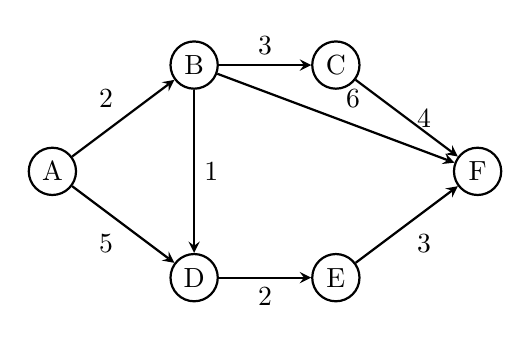
\begin{tikzpicture}[
    vertex/.style={circle, draw, minimum size=6mm, inner sep=0pt},
    >=stealth, thick, scale=0.9
  ]
  \node[vertex] (A) at (0,1.5) {A};
  \node[vertex] (B) at (2,3) {B};
  \node[vertex] (C) at (4,3) {C};
  \node[vertex] (D) at (2,0) {D};
  \node[vertex] (E) at (4,0) {E};
  \node[vertex] (F) at (6,1.5) {F};
  \draw[->] (A) -- node[above left] {2} (B);
  \draw[->] (A) -- node[below left] {5} (D);
  \draw[->] (B) -- node[above] {3} (C);
  \draw[->] (B) -- node[right] {1} (D);
  \draw[->] (C) -- node[right] {4} (F);
  \draw[->] (D) -- node[below] {2} (E);
  \draw[->] (E) -- node[below right] {3} (F);
  \draw[->] (B) -- node[above right] {6} (F);
\end{tikzpicture}
\end{center}
\end{exercice}

\begin{exercice}[$\star\star$ -- Bellman-Ford]
Appliquer Bellman-Ford au m\^eme graphe en ajoutant l'arc $(E, B)$ de poids
$-4$.  D\'etecter s'il y a un cycle n\'egatif.
\end{exercice}

\begin{exercice}[$\star\star$ -- Floyd-Warshall]
Calculer la matrice des plus courtes distances pour un graphe complet \`a 4
sommets de votre choix.
\end{exercice}

\begin{exercice}[$\star\star$ -- Kruskal et Prim]
Trouver l'ACM du graphe suivant par les deux m\'ethodes et v\'erifier qu'on
obtient le m\^eme r\'esultat~:
\begin{center}
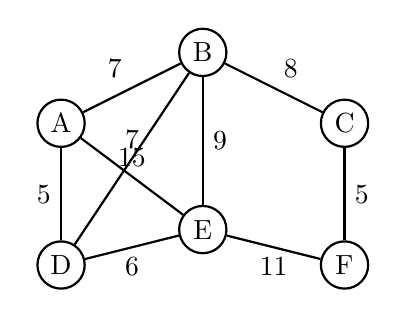
\begin{tikzpicture}[
    vertex/.style={circle, draw, minimum size=6mm, inner sep=0pt},
    thick, scale=0.9
  ]
  \node[vertex] (A) at (0,2) {A};
  \node[vertex] (B) at (2,3) {B};
  \node[vertex] (C) at (4,2) {C};
  \node[vertex] (D) at (0,0) {D};
  \node[vertex] (E) at (2,0.5) {E};
  \node[vertex] (F) at (4,0) {F};
  \draw (A) -- node[above left] {7} (B);
  \draw (A) -- node[left] {5} (D);
  \draw (B) -- node[above right] {8} (C);
  \draw (B) -- node[right] {9} (E);
  \draw (C) -- node[right] {5} (F);
  \draw (D) -- node[below] {6} (E);
  \draw (E) -- node[below] {11} (F);
  \draw (A) -- node[above] {15} (E);
  \draw (B) -- node[above] {7} (D);
\end{tikzpicture}
\end{center}
\end{exercice}

\begin{exercice}[$\star\star\star$ -- PERT/CPM]
Un projet comporte les t\^aches suivantes~:
\begin{center}
\begin{tabular}{cccc}
  \toprule
  T\^ache & Dur\'ee & Pr\'ed\'ecesseurs \\
  \midrule
  A & 3 & -- \\
  B & 5 & A \\
  C & 2 & A \\
  D & 4 & B, C \\
  E & 6 & C \\
  F & 2 & D, E \\
  \bottomrule
\end{tabular}
\end{center}
Construire le graphe, trouver le chemin critique et la dur\'ee minimale du
projet.
\end{exercice}
